%
% $Id: blank.tex,v 2.0 2010-01-05 18:50:50+09 kobayasi Exp $
%
% Mar 21, 2001:  Revision Control Started!!
%
\documentclass[11pt]{jarticle}
\usepackage{newcent}             % PDFへの変換後の品質を高める
%
%\usepackage[doctor]{gaiyo}      % 博士論文要旨の場合
\usepackage[master]{gaiyo}      % 修士論文要旨の場合
%\usepackage{gaiyo}               % 卒業研究概要の場合
%\usepackage[junior]{gaiyo}      % 専門演習レポートの場合

%\usepackage{graphicx}
\usepackage[dvipdfmx]{graphicx}
\usepackage{epsf}
\usepackage{comment}

\title{複数の携帯端末による教室空間の空間音響環境構築手法の検討}
\id{14M7102}
\author{伊納洋佑}
\teacher{米澤朋子}

\begin{document}
\maketitle

\section{はじめに}

近年,スマートフォンやタブレット,ノートパソコンなどの高度な計算能力とネットワーク接続が可能なスマートデバイスが普及し,インターネットへの常時接続が可能になった.
こうした流れを受け,これらのスマートデバイスを互いに協調的に制御する研究が盛んになってきている\cite{shibata14}.
しかしながら,これらはセンシング技術が主体であり,環境に存在する人間に働きかけるものは少ない.
そこで本研究は,室内空間において,各々の所有するスマートデバイスを用いて平面配置のスピーカアレイを構築し,音像定位を行うシステムを開発した.
このシステムは
例えば,授業中の生徒のスマートデバイスを用いることで,教室の特定の人間グループに対して注意喚起を促すことができる.
他にも,音像位置を動かすような効果を与えることができるので,音を用いた様々な活動に使えると考えられる.

\section{提案システム}

本システムは多端末の時刻同期と測距を音声パルスで実現し,端末のスピーカを用いた音像定位を実現する.


まず,スマートデバイスのスピーカを用いた音像定位手法として,仮想音源と各スピーカとの距離から距離減衰を算出し振幅による音像定位をするDBAP法を用いた\cite{dbap}.
これを用いてデバイス間で指定音源位置から音を鳴らすためには,遅延のないよう端末間同期,仮想音源と各端末間の距離推定,
および各スピーカ間の音圧レベル制御が必要である.


スマートデバイスやセンサネットワークなどでの時刻同期の手法として,音声パルスの往復による時刻同期手法が提案されている\cite{tpsn}.
二つの端末間で音声パルスを交互に鳴らし,互いの端末でのパルスの到来時刻から標準大気圧下での音速における伝搬時間の差を利用し相対距離を求める.
この手法を用い,各端末が一回ずつ音声パルスを鳴らし互いのパルスの到来時刻とその差を計測し,時刻同期と相対距離計測を行った.


上記の手法で判明した各端末の相対距離から,非計量多次元尺度構成法を用いて空間上での相対的な分布を推定することで,
距離測定誤差があったり距離が離れすぎていて音声パルス検出に失敗する場合にも対応しようと考えた.
非計量多次元尺度法では,計測相対距離と推定位置の相対距離の差を取る誤差関数を最少化する非線形最適化問題として定式化し,最急降下法で解く.


高精度な測距には,パルスの到来時刻の正確な検出が必要である.その一方室内環境は環境雑音や壁や天井などに反射によるマルチパスによる問題が生じる.
そこで,環境雑音にも強い擬似雑音系列を用いた直接スペクトル拡散方式によるパルス圧縮を音声パルスに用いた.
そしてマルチパス環境下でのパルス位置推定手法として,Rake 受信器にも使われる伝送路測定用信号と計測信号の二つを用意する手法を応用し,
それらの信号を互いに短時間相互相関にかけることで,厳密なパルス到来時刻の同定を試みた.


音源定位においては,異種端末間でのハードウェア・ソフトウェアに起因する差異の影響を考慮する必要がある.
例えば,スピーカ出力やシステムクロックの異なる端末間では, DBAP 法の適用上問題や同期後の時間経過による同期ズレ発生の問題がある.
このような端末間差異の校正手法としてスピーカ出力に関しては同期信号の距離減衰から各端末の相対音圧を推定する手法を,
同期ズレに対しては一定時間後に再同期することでクロック差を検出する手法を検討した.


これらの制御システムとして,通信を中継する中央サーバと計算サーバを導入したスター型ネットワーク構成と, P2P リングネットワークによる構成の二つを提案した.


\section{検証}
本手法における端末間距離測定を評価した.MacBookPro13 インチ 4 台を,図\ref{fig:relpos}に配置し,先述 のアルゴリズムにより各端末間距離を 50 回計測した結果を図\ref{tab:estdistance}に示す.
計測された各端末間の信号伝達時間と音速 を 340m/s と仮定したときの計測距離より,誤差は平均で30cm程度となりDBAP法での音源生成には問題が生じない程度の精度を得られた.

\section{おわりに}
本稿では,多数の人間が存在する室内空間に音源定位した複数の音を配置し用いることを考え,
音像定位を行なうシステムを開発した.
各自が所有するスマートデバイスを用いて平面配置のスピーカアレイを構築し,
所望の位置に音源配置した音声情報を提供するシステムを提案した.
この手法を用いて発生させた音は,3 つの発音端末の三角形の外の受聴者には三角形内に定位されることを確認した.
今後は,各端末の特性としてマイクやスピーカ位置,音響特性を考慮することや,端末数をどの程度まで増やすべきかの議論を行っていきたい.

\begin{figure}[htbp]
  \begin{center}
    \begin{tabular}{c}
      \begin{minipage}{0.4\hsize}
        \begin{center}
          \hspace{-2mm}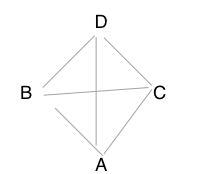
\includegraphics[clip,width=0.7\hsize]{img/PC_haichi.png}
          \caption{PC配置}
          \label{fig:relpos}
        \end{center}
      \end{minipage}
      \begin{minipage}{0.58\hsize}
        \begin{center}
          \begin{tabular}{l|rrrrr}
            \hline
            {\footnotesize  端末間}&{\footnotesize 平均}&{\footnotesize 標準偏差}&{\footnotesize 実測距離(m) }\\
            \hline
            {\footnotesize A-D }&{\footnotesize 11.71889953}&{\footnotesize 1.24793883}&{\footnotesize 11.10 }\\
            {\footnotesize B-D }&{\footnotesize 7.767573696}&{\footnotesize 0.583510141}&{\footnotesize 7.77 }\\
            {\footnotesize C-D }&{\footnotesize 6.72675737}&{\footnotesize 0.774180135}&{\footnotesize 6.72 }\\
            {\footnotesize A-B }&{\footnotesize 6.564537924}&{\footnotesize 1.067679838}&{\footnotesize 6.83 }\\
            {\footnotesize A-C }&{\footnotesize 7.300425749}&{\footnotesize 1.283308926}&{\footnotesize 6.93 }\\
            {\footnotesize B-C }&{\footnotesize 4.771470221}&{\footnotesize 0.664454607}&{\footnotesize 4.92 }\\
            \hline
          \end{tabular}
          \caption{50回試行時の端末間距離計測結果}
          \label{tab:estdistance}
        \end{center}
      \end{minipage}
    \end{tabular}
  \end{center}
\end{figure}




\begin{thebibliography}{10}

\bibitem{shibata14} 柴田一暁, 小野順貴, 亀岡弘和. 音の発信を利用したキャリブレーションに基づくアドホックマイクロホンアレイによる音源定位. 音講論 (春), pp. 707--710,2014.
\bibitem{dbap}      Trond Lossius, Pascal Baltazar, and Theo de la Hogue. DBAP–distance-based amplitude panning. Proc of ICMC 2009, pp.489--492, 2009.
\bibitem{tpsn}      S. Ganeriwal, R. Kumar, Ram, M.B. Srivastava. Timing-sync protocol for sensor networks. In Proceedings of the 1st international conference on Embedded networked sensor systems. ACM,  pp. 138-149, 2003.

\end{thebibliography}

\end{document}
